\documentclass[10pt]{article}
\usepackage[letterpaper, margin = 0.75 in]{geometry}
\usepackage{amsmath,amsthm,amssymb, graphicx, wrapfig, multirow,float, setspace,titlesec}
\usepackage{listings}
\titleformat*{\section}{\fontsize{15}{20}\selectfont}
\titleformat*{\subsection}{\fontsize{12}{17}\selectfont}

\renewcommand{\floatpagefraction}{0.9}
\renewcommand{\textfraction}{0.25}

\newcommand{\N}{\mathbb{N}}
\newcommand{\Z}{\mathbb{Z}}

 
\begin{document}
 
\title{Ph20 - Assignment 4}
\author{Mai H Nguyen}
\date{14 May 2018}
 
\maketitle
\section{Version control log}
\lstinputlisting[language=Python]{log.txt}

\section {Makefile}
\lstinputlisting[language=Python]{makefile.sh}

\section{Modification to source code}
\subsection{Load code}
\lstinputlisting[language=Python]{load.py}

\subsection{Modifications to existing codes to generate graphs}
\begin{lstlisting}[language=Python]
import sys
from load import *

def spring(input_file, output_file):
    [x0, v0, t, h] = load_num(input_file)

if __name__ == '__main__':
    input_file = sys.argv[1]
    output_file = sys.argv[2]
    spring(input_file, output_file)
\end{lstlisting}

\section{Graphs generated by makefile}
Command-line inputs for separate plots
\begin{lstlisting}[language=bash]
$ make A311.png
$ make A313_trunc_t.png
$ make A313_trunc_x.png
$ make A315_comp.png
$ make A321_comp.png
$ make A323_comp.png
$ make A324.png
\end{lstlisting}
\begin{figure}
\centering
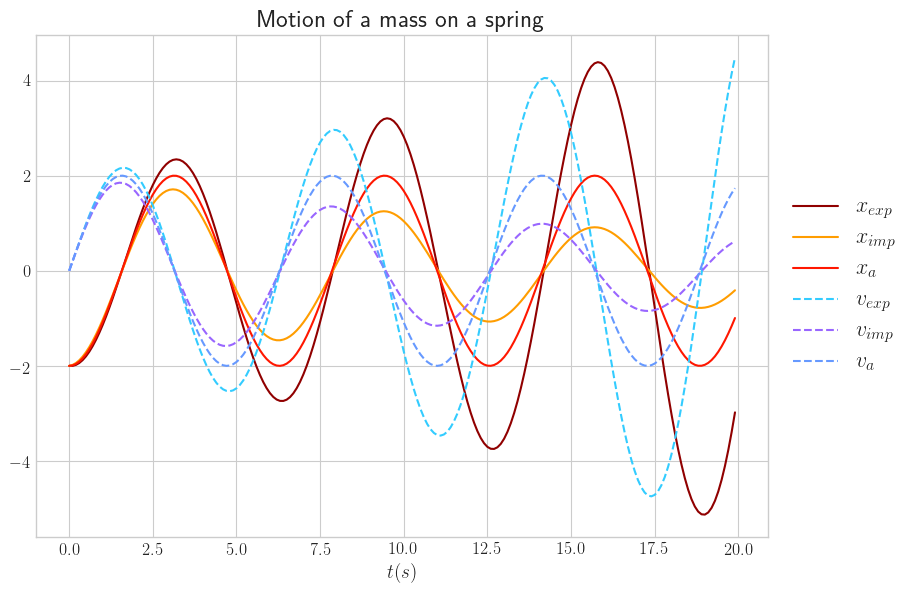
\includegraphics[width=0.48\textwidth]{A311.png}
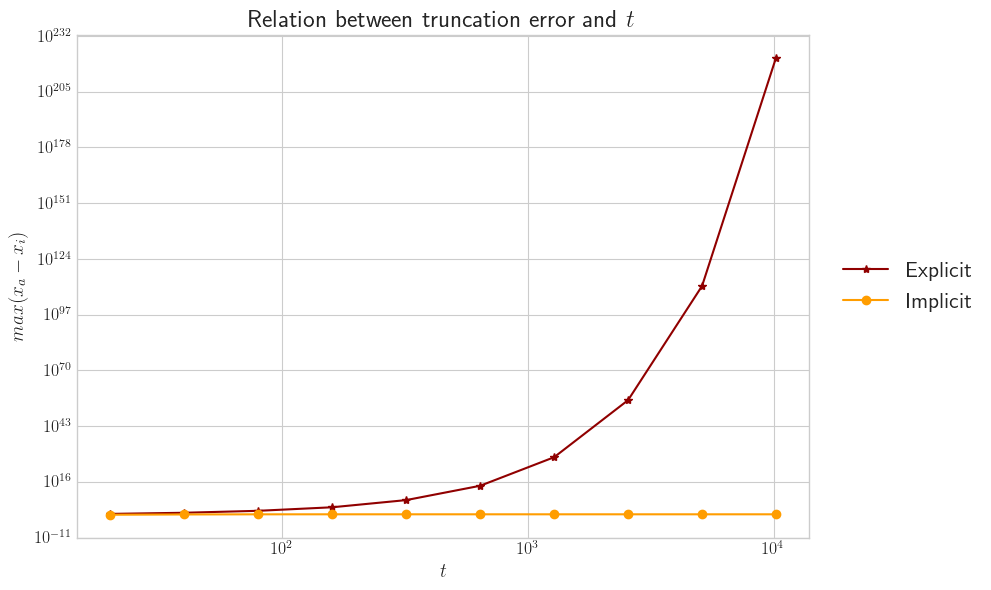
\includegraphics[width=0.48\textwidth]{A313_trunc_t.png}
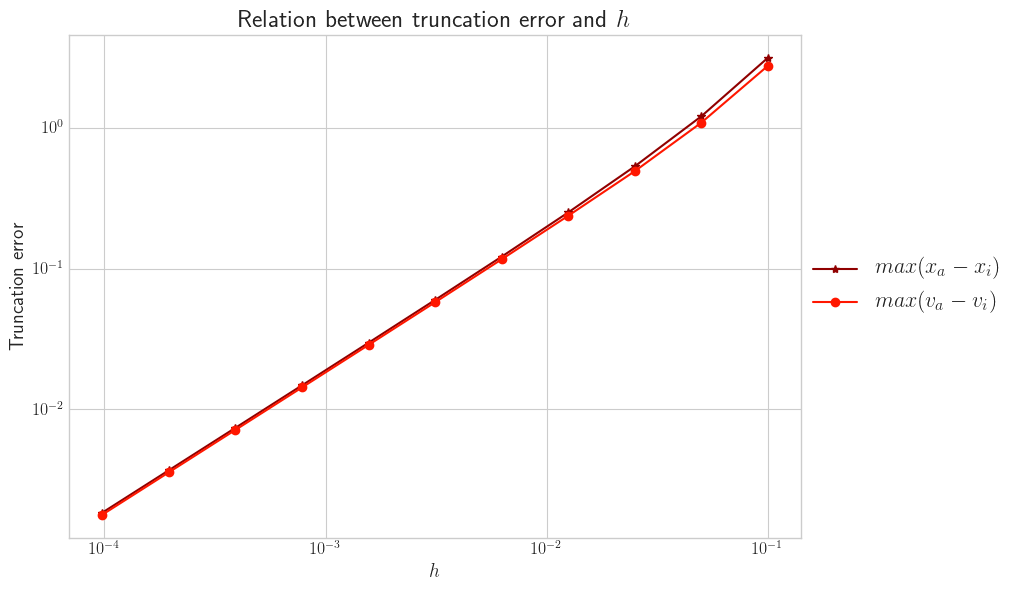
\includegraphics[width=0.48\textwidth]{A313_trunc_x.png}
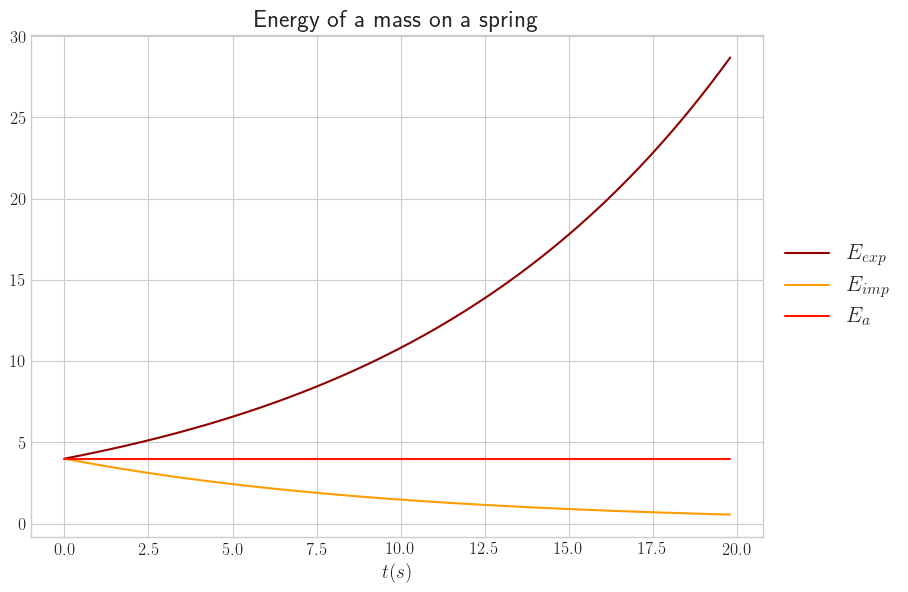
\includegraphics[width=0.48\textwidth]{A315_comp.png}
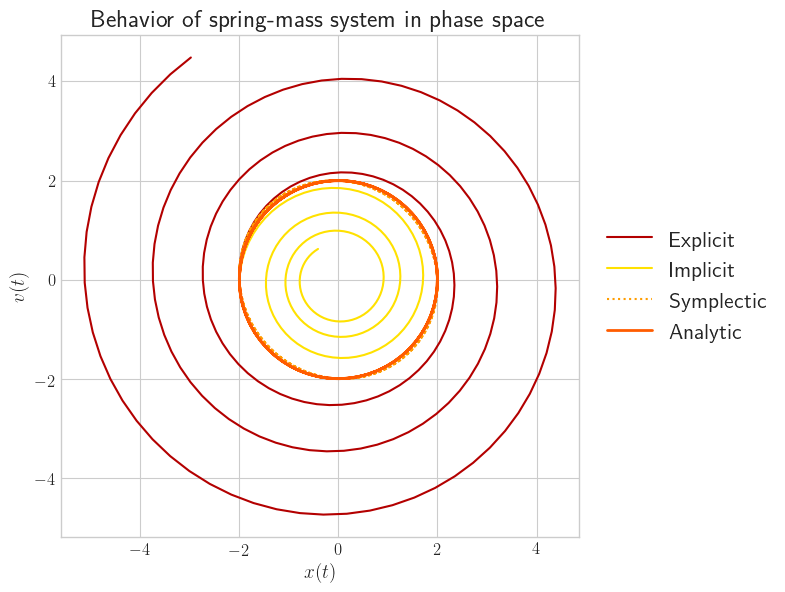
\includegraphics[width=0.48\textwidth]{A321_comp.png}
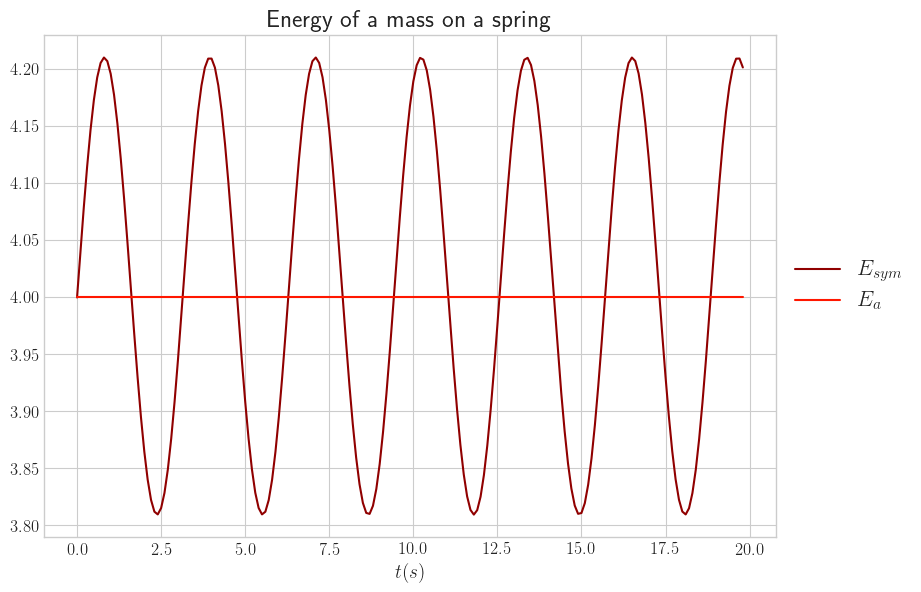
\includegraphics[width=0.48\textwidth]{A323_comp.png}
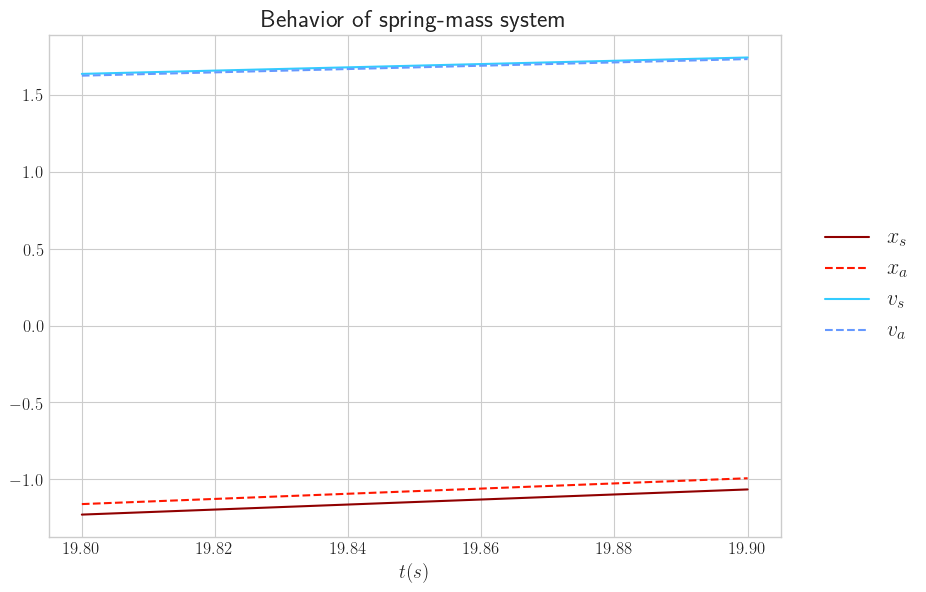
\includegraphics[width=0.48\textwidth]{A324.png}
\end{figure}

\end{document}
